\documentclass{article}
\usepackage[letterpaper,top=2cm,bottom=2cm,left=3cm,right=3cm,marginparwidth=1.75cm]{geometry}

\usepackage{amsmath}
\usepackage{graphicx}
\usepackage[colorlinks=true, allcolors=blue]{hyperref}
\usepackage{listings}

\begin{document}
\begin{titlepage}
\centering
\begin{figure}
\centering
{\bfseries\LARGE Escuela técnica superior\par}
{\scshape\Large Facultad de Ingeniería Informática\par}
\vspace{5cm}
\centering

\includegraphics[scale=0.25]{img/img1.png} 
\end{figure}


{\scshape\Huge Práctica 6\par}
{\scshape\Large Servidor de correo\par}
\vspace{9cm}
{\Large Ignacio Fernández Contreras\par}
\vfill
\end{titlepage}
\clearpage\hbox{}\thispagestyle{empty}\newpage

\section{Enunciado}
Deseamos instalar un servidor de correo electrónico (solo local). Para ello queremos utilizar Postfix
y Dovecot. Se pide:
\begin{enumerate}
\item Describir paso a paso el proceso de instalación y configuración del servidor de correo con Postfix y Dovecot. 
\item Probar que el servidor de correo funciona correctamente con un cliente de correo o
utilizando Telnet. 
\item Instalar y configurar RoundCube, describiendo los pasos realizados.
\end{enumerate}


\section{¿Qué es Postfix?}
Postfix es un servidor de transferencia de correo (MTA, por sus siglas en inglés) de código abierto. En esencia, es un programa de software que se utiliza para enrutamiento y entrega de correo electrónico en sistemas basados en Unix o Linux. Postfix fue desarrollado por Wietse Venema y está diseñado para ser una alternativa más rápida, segura y fácil de administrar en comparación con el servidor de correo Sendmail, que era muy popular pero a menudo considerado más complejo.\\

Las funciones principales de Postfix incluyen:\\
\begin{enumerate}
\item \textbf{Transferencia de Correo}: Postfix se encarga de recibir correos electrónicos del cliente de envío (a través del protocolo SMTP) y de enrutarlos hacia su destino, ya sea en el mismo servidor o hacia otros servidores de correo.
\item \textbf{Seguridad}: Postfix se ha diseñado con un enfoque en la seguridad. Implementa diversas características para prevenir abusos, como protección contra retransmisiones de correo no autorizadas, filtrado de spam y soporte para conexiones seguras mediante TLS (Transport Layer Security).
\item \textbf{Configuración Flexible}: Postfix es conocido por su configuración flexible y su capacidad para integrarse con otros componentes del sistema de correo electrónico. Puede funcionar junto con servidores IMAP/POP3 como Dovecot para permitir a los usuarios acceder a sus buzones de correo.
\item \textbf{Mantenimiento y Escalabilidad}: Postfix es fácil de administrar y es escalable para manejar grandes volúmenes de correo. Además, se preocupa por la eficiencia en el procesamiento de correos electrónicos, lo que contribuye a su rendimiento y confiabilidad.
\end{enumerate}

\section{¿Qué es Dovecot?}
Dovecot es un servidor de correo electrónico de código abierto que proporciona servicios de acceso a buzones de correo en servidores que utilizan los protocolos IMAP (Internet Message Access Protocol) y POP3 (Post Office Protocol 3). Su función principal es permitir a los usuarios recuperar y gestionar sus correos electrónicos almacenados en un servidor.\\

Las funciones principales de Dovecot incluyen:\\
\begin{enumerate}
\item \textbf{Acceso IMAP y POP3}: Dovecot permite a los clientes de correo electrónico conectarse al servidor y recuperar mensajes a través de los protocolos IMAP y POP3. IMAP es especialmente útil, ya que permite a los usuarios organizar, marcar y gestionar sus correos electrónicos en el servidor, lo que facilita el acceso desde múltiples dispositivos.
\item \textbf{Seguridad}: Dovecot se preocupa por la seguridad de la comunicación entre el cliente y el servidor. Puede integrarse con protocolos seguros como TLS/SSL para cifrar la conexión, protegiendo así la confidencialidad de la información transmitida.
\item \textbf{Integración con otros componentes de correo}: Dovecot suele utilizarse junto con otros componentes de software de servidor de correo electrónico, como Postfix (un servidor de transferencia de correo), para proporcionar un sistema de correo electrónico completo y funcional.
\item \textbf{Soporte para múltiples autenticaciones}: Dovecot es flexible en términos de autenticación y puede integrarse con varios sistemas de autenticación, como archivos de contraseñas locales, bases de datos SQL o incluso sistemas de autenticación externos.
\end{enumerate}


\section{Ejercicio 1}
\subsection{Instalación de Postfix}
Antes de empezar con cualquier instalacion:

\lstset{language=Bash, breaklines=true, basicstyle=\footnotesize}
\begin{lstlisting}[frame=single]
sudo apt update
sudo apt upgrade
\end{lstlisting}

Una vez actualizado nuestro sistema, procedemos a intalar Postfix y Dovecot:
\lstset{language=Bash, breaklines=true, basicstyle=\footnotesize}
\begin{lstlisting}[frame=single]
sudo apt install postfix dovecot-core dovecot-imapd dovecot-pop3d
\end{lstlisting}
Durante la instalación de Postfix, selecciona "Sitio de Internet" y deja el resto por defecto.
\begin{center}
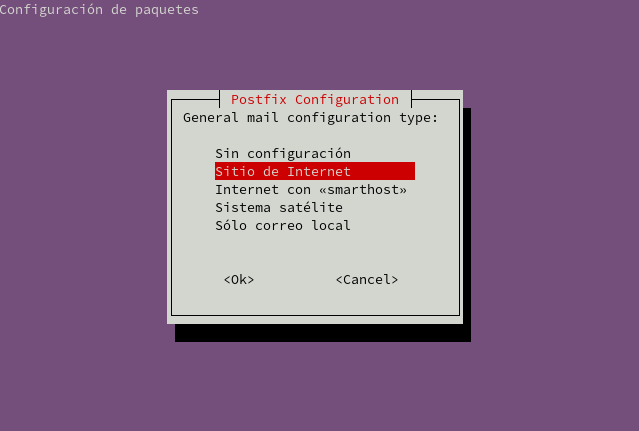
\includegraphics[scale=0.4]{img/img2.png} 
\end{center}

 

Ahora, vamos a configurarlo:
\lstset{language=Bash, breaklines=true, basicstyle=\footnotesize}
\begin{lstlisting}[frame=single]
sudo nano /etc/postfix/main.cf
\end{lstlisting}

Agregando las siguientes lineas
\lstset{language=Bash, breaklines=true, basicstyle=\footnotesize}
\begin{lstlisting}[frame=single]
myhostname = pagina1
mydomain = pagina1.com
myorigin = $pagina1
home_mailbox = Maildir/
\end{lstlisting}

Una vez configurado, reiniciamos postfix:
\lstset{language=Bash, breaklines=true, basicstyle=\footnotesize}
\begin{lstlisting}[frame=single]
sudo systemctl restart postfix
\end{lstlisting}


\subsection{Configuración de Dovecot}
Una vez configurado, reiniciamos postfix:
\lstset{language=Bash, breaklines=true, basicstyle=\footnotesize}
\begin{lstlisting}[frame=single]

sudo nano /etc/dovecot/dovecot.conf
\end{lstlisting}

Añadimos las siguientes lineas:
\lstset{language=Bash, breaklines=true, basicstyle=\footnotesize}
\begin{lstlisting}[frame=single]
protocols = imap pop3
mail_location = maildir:~/Maildir
auth_mechanisms = plain login
\end{lstlisting}


\section{Ejercicio 2}
\subsection{¿Qué es Telnet?}
Telnet es un protocolo de red que permite la comunicación bidireccional a través de una conexión de terminal virtual. También se refiere a la aplicación de software utilizada para implementar este protocolo. La función principal de Telnet es permitir que un usuario se conecte a un servidor remoto y acceda a recursos y servicios como si estuviera directamente conectado al sistema remoto.

Telnet funciona a través de una red, como Internet, y utiliza el protocolo TCP (Transmission Control Protocol) para establecer la conexión. Una vez establecida la conexión, Telnet permite a los usuarios enviar comandos al sistema remoto y recibir las respuestas. Esto hace que sea posible realizar tareas administrativas, configurar dispositivos de red, acceder a recursos compartidos y realizar diversas operaciones en sistemas remotos.

Es importante destacar que, aunque Telnet ha sido ampliamente utilizado en el pasado, su uso ha disminuido debido a problemas de seguridad. La información transmitida a través de Telnet, incluyendo contraseñas y otros datos sensibles, se envía en texto no cifrado, lo que hace que sea vulnerable a la interceptación y el acceso no autorizado. Por esta razón, se recomienda utilizar protocolos más seguros, como SSH (Secure Shell), que cifran la comunicación para proteger la privacidad y la seguridad de la información transmitida.
\\

Vamos a comprobar si funciona:

\lstset{language=Bash, breaklines=true, basicstyle=\footnotesize}
\begin{lstlisting}[frame=single]
telnet localhost 25
\end{lstlisting}

\begin{center}
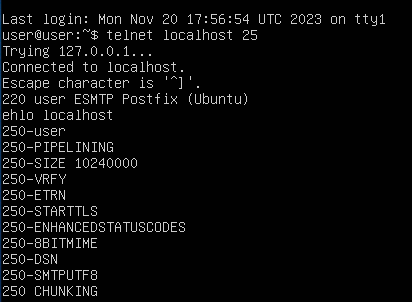
\includegraphics[scale=0.6]{img/img4.png} 
\end{center}
 

Verificamos de igual forma, si Dovecot funciona:
\lstset{language=Bash, breaklines=true, basicstyle=\footnotesize}
\begin{lstlisting}[frame=single]
telnet localhost 110
\end{lstlisting}

\begin{center}
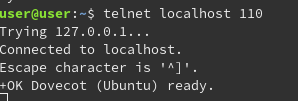
\includegraphics[scale=0.6]{img/img5.png} 
\end{center}
\lstset{language=Bash, breaklines=true, basicstyle=\footnotesize}
\begin{lstlisting}[frame=single]
telnet localhost 143
\end{lstlisting}
\begin{center}
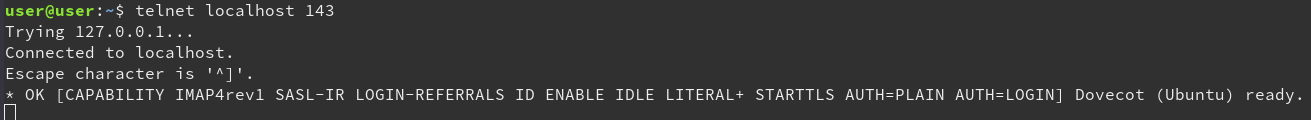
\includegraphics[width=\textwidth]{img/img6.png} 
\end{center}


\section{Ejercicio 3}
\subsection{¿Qué es RoundCube?}

Roundcube es un cliente de correo electrónico de código abierto que proporciona una interfaz web para acceder y gestionar correos electrónicos. Es una aplicación de software que permite a los usuarios enviar, recibir y organizar sus mensajes de correo electrónico a través de un navegador web. Roundcube se destaca por ser fácil de usar y ofrece una interfaz intuitiva para las funciones comunes de correo electrónico, como la lectura, redacción, envío y organización de mensajes.\\


Entre sus características, Roundcube suele incluir la capacidad de organizar correos electrónicos en carpetas, buscar mensajes, adjuntar archivos, gestionar contactos y configurar preferencias de cuenta. Además, es compatible con estándares de correo electrónico como IMAP y SMTP.\\


Es importante tener en cuenta que Roundcube es el cliente de correo electrónico, mientras que el servidor de correo (como Postfix mencionado anteriormente) es responsable de gestionar la entrega y recepción de los correos electrónicos. En conjunto, un servidor de correo y un cliente como Roundcube permiten a los usuarios enviar, recibir y administrar sus correos electrónicos de manera efectiva.

\subsection{Instalación de RoundCube}
\lstset{language=Bash, breaklines=true, basicstyle=\footnotesize}
\begin{lstlisting}[frame=single]
sudo apt install roundcube roundcube-mysql
\end{lstlisting}
Vamos ahora, a configurar mysql
\lstset{language=Bash, breaklines=true, basicstyle=\footnotesize}
\begin{lstlisting}[frame=single]
create user 'roundcube_user'@'localhost' identified by 'user';
grant all privileges on roundcubemail.* to 'roudcube_user'@'localhost' with grant option;
flush privileges;
\end{lstlisting}

\subsection{Configuración de RoundCube}
\lstset{language=Bash, breaklines=true, basicstyle=\footnotesize}
\begin{lstlisting}[frame=single]
wget https://github.com/roundcube/roundcubemail/releases/download/1.4.9/roundcubemail-1.4.9- complete.tar.gz
\end{lstlisting}

Descomprimir el fichero en /var/www:
\lstset{language=Bash, breaklines=true, basicstyle=\footnotesize}
\begin{lstlisting}[frame=single]
sudo tar -xvf roundcubemail-1.4.9-complete.tar.gz -C /var/www
\end{lstlisting}

Renombramos la carpeta a "roundcube":
\lstset{language=Bash, breaklines=true, basicstyle=\footnotesize}
\begin{lstlisting}[frame=single]
cd /var/www
sudo mv roundcubemail-1.4.9 roundcube
\end{lstlisting}

Cambiamos el propietario
\lstset{language=Bash, breaklines=true, basicstyle=\footnotesize}
\begin{lstlisting}[frame=single]
chown -R www-data:www-data roundcube
\end{lstlisting}

Cambiamos los permisos de la carpeta:
\lstset{language=Bash, breaklines=true, basicstyle=\footnotesize}
\begin{lstlisting}[frame=single]
sudo chmod 775 -R roundcube/logs roundcube/temp
\end{lstlisting}
En la carpeta sites-available de Apache, crear un fichero roundcube.conf y configurarlo, por ejemplo, de la siguiente manera:
\lstset{language=Bash, breaklines=true, basicstyle=\footnotesize}
\begin{lstlisting}[frame=single]
<VirtualHost *:80>
	ServerName correo.ejemplo.uma
	ServerAdmin admin@ejemplo.uma
	DocumentRoot /var/www/roundcube
</VirtualHost> 
\end{lstlisting}

Habilitamos el nuevo sitio y el módulo rewrite
\lstset{language=Bash, breaklines=true, basicstyle=\footnotesize}
\begin{lstlisting}[frame=single]
sudo a2ensite roundcube
sudo a2enmod rewrite
sudo systemctl restart apache2
\end{lstlisting}
Vamos a configurar mysql
\lstset{language=Bash, breaklines=true, basicstyle=\footnotesize}
\begin{lstlisting}[frame=single]
create database roundcubemail
create user 'roundcube'@ 'localhost' identified by 'claveroundcube';
grant all privileges on roundcubemail.* to 'roundcube'@'localhost';
flush privileges;
\end{lstlisting}

\begin{center}
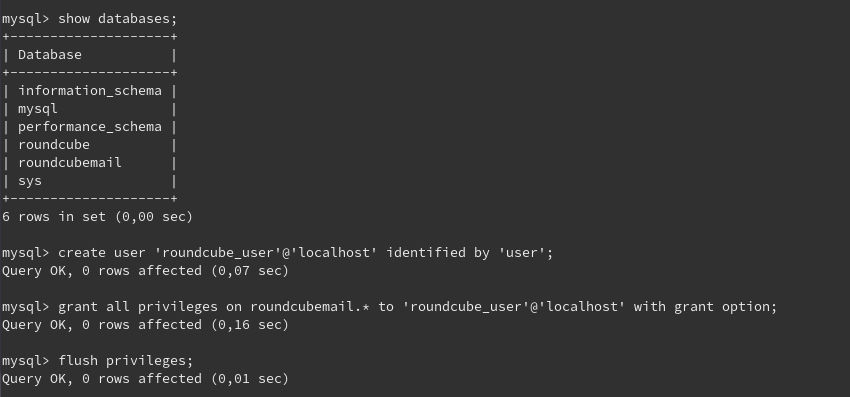
\includegraphics[scale=0.4]{img/Screenshot from 2023-11-20 19-20-42.png} 
\end{center}

Añadimos la información necesaria a la base de datos de roundcube
\lstset{language=Bash, breaklines=true, basicstyle=\footnotesize}
\begin{lstlisting}[frame=single]
sudo mysql roundcubemail < /var/www/roundcube/SQL/mysql.initial.sql
\end{lstlisting}

\begin{center}
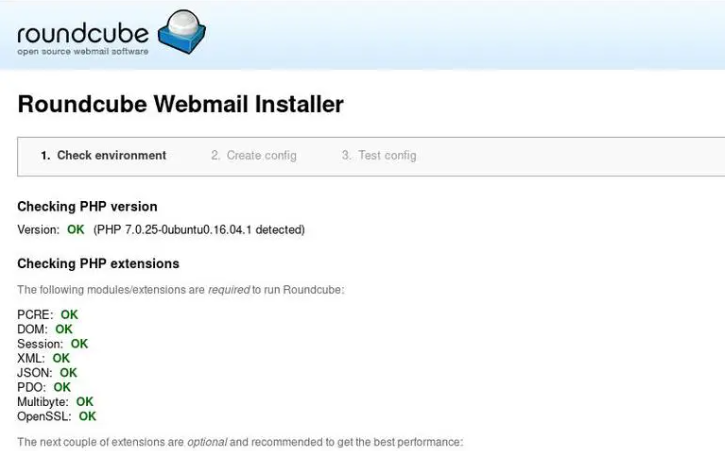
\includegraphics[scale=0.5]{img/img7.png} 
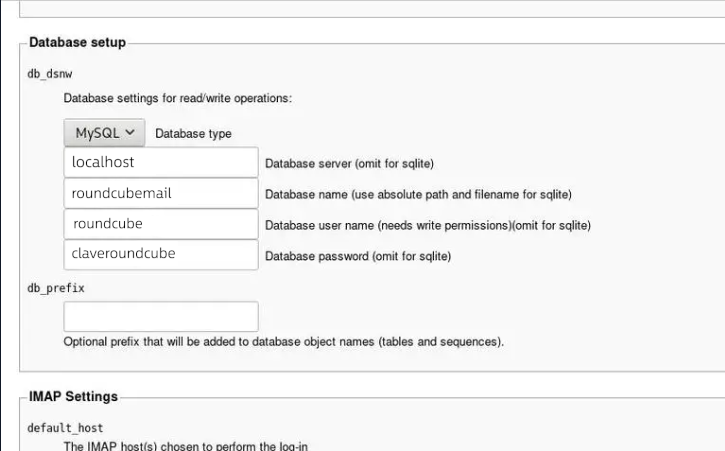
\includegraphics[scale=0.5]{img/img8.png} 
\end{center}




\end{document}